
\tikzstyle{startstop} = [rectangle, rounded corners, text centered, draw=black, fill=red!30]
\tikzstyle{process} = [rectangle, text centered, draw=black, fill=orange!30]
\tikzstyle{decision} = [rectangle, text centered, draw=black, fill=green!30]
\tikzstyle{arrow} = [thick,->,>=stealth]

\framebox{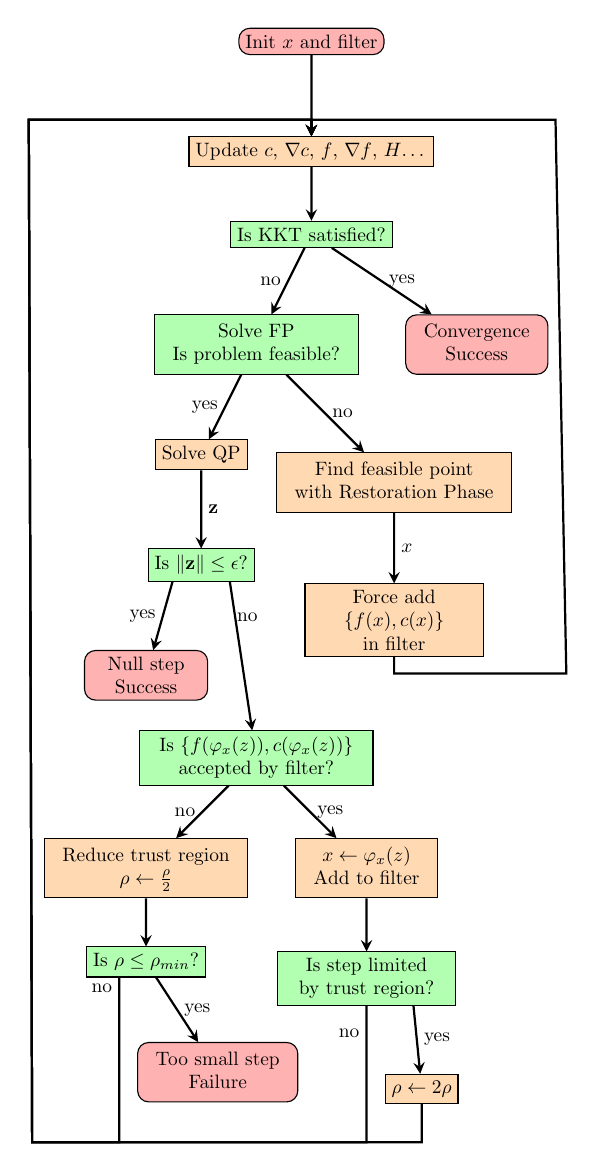
\begin{tikzpicture}[node distance=2cm, scale=0.7, every node/.style={transform shape}]

\node (init) [startstop] {Init $x$ and filter};
\node (update) [process, below of=init] {Update $c$, $\nabla c$, $f$, $\nabla f$, $H$\ldots};
\node (KKT) [decision, below of=update, yshift=0.5cm] {Is KKT satisfied?};
\node (success) [startstop, below of=KKT, xshift=3cm] {\begin{tabular}{c}Convergence\\ Success\end{tabular}};
\node (FP) [decision, below of=KKT, xshift=-1cm] {\begin{tabular}{c}Solve FP\\ Is problem feasible?\end{tabular}};
\node (QP) [process, below of=FP, xshift=-1cm] {Solve QP};
\node (restoration) [process, below of=FP, xshift=25mm, yshift=-0.5cm] {\begin{tabular}{c}Find feasible point\\ with Restoration Phase\end{tabular}};
\node (forceAdd) [process, below of=restoration, text width=3cm, yshift=-0.5cm] {Force add $\{f(x),c(x)\}$ in filter};
\node (zeroStep) [decision, below of=QP] {Is $\|\mathbf{z}\| \leq \epsilon$?};
\node (success2) [startstop, below of=zeroStep, xshift=-1cm, text width=2cm] {Null step Success};
\node (filterTest) [decision, below of=zeroStep, text width=4cm, yshift=-1.5cm, xshift=1cm] {Is $\{f(\varphi_x(z)),c(\varphi_x(z))\}$ accepted by filter?};
\node (reduceTR) [process, below of=filterTest, xshift=-2cm] {\begin{tabular}{c}Reduce trust region\\ $\rho\leftarrow\frac{\rho}{2}$\end{tabular}};
\node (smallStepTest) [decision, below of=reduceTR, yshift=3mm] {Is $\rho \leq \rho_{min}$?};
\node (fail) [startstop, below of=smallStepTest, xshift=13mm, yshift=0mm] {\begin{tabular}{c}Too small step\\
Failure\end{tabular}};
\node (addToFilter) [process, below of=filterTest, xshift=2cm] {\begin{tabular}{c}$x\leftarrow\varphi_x(z)$\\Add to filter\end{tabular}};
\node (limitedStep) [decision, below of=addToFilter, xshift=0mm, yshift=0mm, text width=30mm] {Is step limited by trust region?};
\node (increaseTR) [process, below of=limitedStep, xshift=1cm] {$\rho\leftarrow 2 \rho$};

\draw [arrow] (init) -- (update);
\draw [arrow] (update) -- (KKT);
\draw [arrow] (KKT) -- node[anchor=east] {no} (FP);
\draw [arrow] (KKT) -- node[anchor=west] {yes} (success);
\draw [arrow] (FP) -- node[anchor=east] {yes} (QP);
\draw [arrow] (FP) -- node[anchor=west] {no} (restoration);
\draw [arrow] (restoration) -- node[anchor=west] {$x$} (forceAdd);
\draw [arrow] (QP) -- node[anchor=west] {$\bf z$} (zeroStep);
\draw [arrow] (zeroStep.210) -- node[anchor=east] {yes} (success2);
\draw [arrow] (zeroStep.330) -- node[anchor=west, shift={(-2mm,7mm)}] {no} (filterTest);
\draw [arrow] (filterTest) -- node[anchor=east] {no} (reduceTR);
\draw [arrow] (filterTest) -- node[anchor=west] {yes}  (addToFilter);
\draw [arrow] (reduceTR) -- (smallStepTest);
\draw [arrow] (addToFilter) -- (limitedStep);
\draw [arrow] (smallStepTest) -- node[anchor=west] {yes} (fail);
\draw [arrow] (limitedStep.330) -- node[anchor=west] {yes} (increaseTR);
\draw [arrow] (forceAdd) |-([shift={(15mm,-3mm)}]forceAdd.south east)-- ([shift={(22mm,3mm)}]update.north east)-|(update);
\draw [arrow] (increaseTR) |-([shift={(-64mm,-7mm)}]increaseTR.south west)-- ([shift={(-29mm,3mm)}]update.north west)-| (update);
\draw [arrow] (limitedStep)node[anchor=east, yshift=-10mm] {no} |-([shift={(-64mm,-7mm)}]increaseTR.south west)-- ([shift={(-29mm,3mm)}]update.north west)-| (update);
\draw [arrow] (smallStepTest.210) node[anchor=east, yshift=-2mm] {no}|-([shift={(-64mm,-7mm)}]increaseTR.south west)-- ([shift={(-29mm,3mm)}]update.north west)-| (update);

\end{tikzpicture}}
